\documentclass{standalone}
\usepackage{mintikz}

\colorlet{mydarkblue}{blue!50!black}
\colorlet{myblue}{blue!30}
\colorlet{mydarkred}{red!60!black}
\colorlet{myred}{red!30}
\colorlet{mydarkgreen}{green!60!black}
\colorlet{mygreen}{green!30}
\colorlet{mydarkorange}{yellow!40!red}
\colorlet{myorange}{yellow!80!red}
\colorlet{myyellow}{yellow!80}
\colorlet{mygrey}{black!15}
\colorlet{mydarkgrey}{black!50}

\tikzstyle{bath}=[
  draw=blue!40!black, top color=blue!10, 
  bottom color=blue!20, shading angle=30, thick, rounded corners=1
  ]
\tikzstyle{source}=[
  draw=red!50!black, top color=red!20, 
  bottom color=red!30, shading angle=30, thick, rounded corners=1
  ]
\tikzstyle{conductor}=[
  draw=black!40, top color=black!8, 
  bottom color=black!20, shading angle=30, thick, rounded corners=1
  ]
\tikzstyle{insulator}=[
  draw=yellow!40!red!80, top color=yellow!90!red!80, 
  bottom color=yellow!80!red!80, shading angle=10, thick, rounded corners=1
  ]
\tikzstyle{C1}=[
  draw=black!80!red!70, top color=black!40!red!10, 
  bottom color=black!80!red!20, shading angle=30, thick
  ]
\tikzstyle{C2}=[
  draw=black!90!green!70, top color=black!50!green!8, 
  bottom color=black!90!green!20, shading angle=30, thick
  ]
\tikzstyle{C3}=[
  draw=black!80!yellow!80, top color=black!20!yellow!10, 
  bottom color=black!80!yellow!20, shading angle=30, thick
  ]

\begin{document}
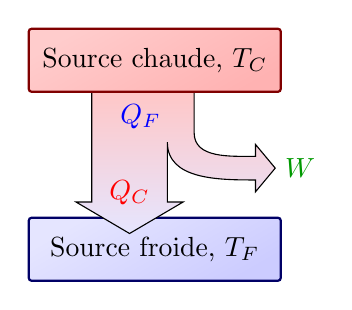
\begin{tikzpicture}
	\def\H{.8}
	\def\W{3.2}
	\def\L{1.6}
	\def\dl{0.0185}
	\coordinate (H) at (0, \L/2);
	\coordinate (C) at (0,-\L/2);

	\draw[bath]
	(C)++(-.4*\W,0) rectangle ++(\W,-\H)
	node[midway,align=center]
		{Source froide, $T_F$};

	\draw[top color=red!22, bottom color=blue!10]
	(H) ++ (-.15*\W,0) -- (-.15*\W,.2-\L/2) --++ (-.2,0) --
	(0,-.2-\L/2) -- (.2+.15*\W,.2-\L/2) --++ (-.2,0) --
	% large arrow: cold reservoir
	(.15*\W,.1*\L) to[out=-90,in=180] (.5*\W,-.2*\L) --++
	(0,-.15) --++ (.25,.3) coordinate (W) --++ (-.25,.3) --++ (0,-.15)
	% small arrow: work
	to[out=180,in=-90] (.5+.1*\W,.2+.05*\L) -- (.5+.1*\W,\L/2);

	\draw[source]
	(H)++(-.4*\W,0)
	rectangle ++(\W,\H)
	node[midway, align=center]
		{Source chaude, $T_C$};

	\node[blue,right=4,below=1] at (H) {$\abs{Q_F}$};
	\node[mydarkgreen,right=0] at (W) {$W$};
	\node[red,above=1] at (C) {$Q_C$};

\end{tikzpicture}
\end{document}
